\documentclass[12pt,a4paper]{article}
\usepackage[margin=1in]{geometry}
\usepackage{hyperref}
\usepackage{graphicx}

\title{\vspace{-1.5cm}COMS30106 Coursework 2 - Identity Crisis}
\author{Ashley Whetter \\ aw0455@bristol.ac.uk
\and
Dominic Moylett \\
dm1905@bristol.ac.uk}
\date{}

\begin{document}
\maketitle
\vspace{-0.5cm}
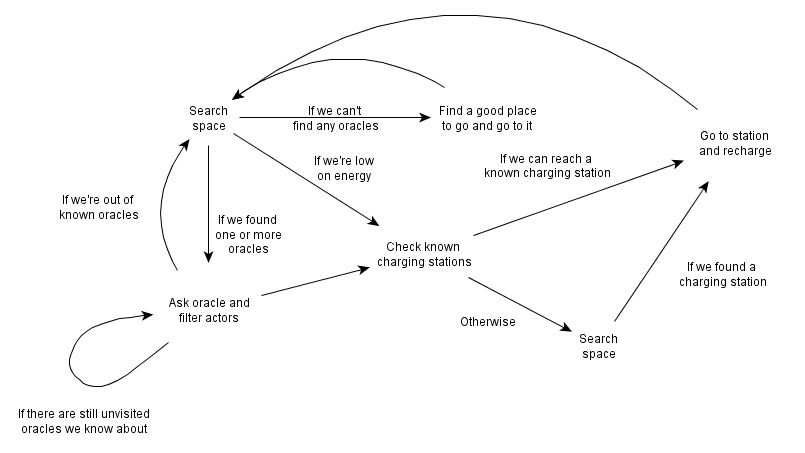
\includegraphics[width=\textwidth]{state_diagram.png}

If the agent is unable to find any new oracles in the search space then it will use all the paths it has found to estimate a good position to go to.
Firstly it will check if any paths end in a position that is in an unsearched area.
This is done by constructing areas around at all the positions it has searched from in the past.
A path is considered a good one to go to if it's end position lies outside of these areas.
Currently we use half the search depth as the radius of the areas.
If none of the paths satisfy this check then it will fall back to randomly picking any of the longest paths,
in the hope that they will take the agent outside of the area that we have just searched.

This strategy works well with the fact that we generally search a block and then
ask every oracle in that block,
because it means that we are more likely to move to areas that we haven't already exhausted.

Any time the agent is in the main search state it will always check whether it needs to recharge first.
The check is a simple threshold.
Ideally this threshold would depend on the maximum amount of energy but that information is not available.
It then goes onto the movement stage.
If during the movement it passes by a charging station and it's energy is below a much higher threshold,
then it will go to that charger and find the new shortest path to the position the oracle was heading to before.

To improve the speed of A* searches we stop searching down paths that have already been visited previously in the current search
because a path that has been found that leads to that position will be shorter than any paths found later.
Ideally we would check if the position has already been searched down by either a bloom filter or a hash table,
but prolog does not have either of these implemented in the standard libraries.
Although we could have used an external language interface to implement one of these data structures in a different language for prolog to use,
instead we decided to just use an associative list,
which has $O(logn)$ lookup time, compared to $O(1)$ of the other data structures mentioned.

\end{document}
